\documentclass[
  % english, % writing in English
  lualatex, % using lualatex for building
  % platex, % building a PDF via a DVI file
  % dvi=dvipdfmx, % building a PDF via a DVI file
]{ipsj-nc}

\usepackage{my_packages}
\usepackage{my_command_definitions}

\title[タイトル]{Title in English}

\author[著者1]{First Author}{Label1}
\author[著者2]{Second Author}{Label1,Label2}

\affiliation
  [所属1]
  {First Affiliation}
  {Label1}
\affiliation
  [所属2]
  {Second Affiliation}
  {Label2}

\begin{document}

\maketitle

% !TEX root = main.tex

\section{出力例}

本章では,章節項や図表,アルゴリズムの出力例を示す.



\subsection{節}

節の出力例.


\subsubsection{項}

項の出力例.

\paragraph{見出し付きパラグラフ}

パラグラフの出力例.



\subsection{図の出力例}

図の出力例を\Fig{\ref{fig:sample}}に示す.

\begin{figure}[t]
  \centering
  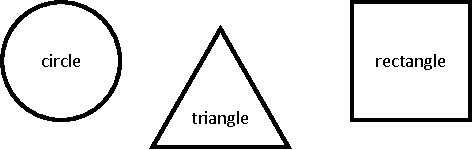
\includegraphics{./figures/sample_figure.pdf}
  \caption{図の例}
  \label{fig:sample}
\end{figure}

以下,図を使用する際の注意点を列挙する.

\paragraph{PDFファイルの使用}

以前は論文をDVIファイルで提出するのが主流だったため図もEPSファイルで作成していたが,現代ではほぼ間違いなくPDFファイルの提出を求められる.
したがって,PowerPointなどで作成した図を直接PDFファイルとして保存し,挿入すればよい.

\paragraph{グレースケールでの表示確認}

PDFファイルでの提出が主流となったため,基本的に図で色を用いても問題ない.
しかし,印刷時に読み手が必ずしもカラー印刷するとは限らないのに加え,人によっては色盲により書き手が色に込めた意図を汲み取れない可能性もある.
そのため,図は始めからグレースケールで作成するか,グレースケールで印刷されても十分に伝わるよう作るべきである.

\paragraph{文字の大きさ}

図を挿入する際にスケールや横幅を操作したために,図中の文字が小さくなってしまうというケースはよくある.
これを防ぐには,初めから論文の大きさに合わせて図を作ってしまうのが簡単である.
基本的にA4二段組の文章であれば横幅8cm文字サイズ8--9ptくらいで作成すればおおよそちょうどよい大きさになる.



\subsection{表の出力例}

\Tab{\ref{tab:sample}}に表の出力例を示す.

\begin{table}[t]
  \caption{表の例(\texttt{booktabs.sty}使用)}
  \label{tab:sample}
  \centering \small
  \begin{tabular}{ccc}
    \toprule
    (1:1)                     & \multicolumn{2}{c}{(1:2--3)}         \\
    \cmidrule(r){1-1}\cmidrule(l){2-3}
    \multirow{2}{*}{(2--3:1)} & (2:2)                        & (2:3) \\
                              & (3:2)                        & (3:3) \\
    \bottomrule
  \end{tabular}
\end{table}

表に関しては,\texttt{booktabs.sty}の使用を勧める.
基本的に表は罫線を少なくする方が見やすいが,{\LaTeXe}標準の表では列の境目を縦の罫線で表すしかない.
一方で,\texttt{booktabs.sty}は列の境目を横罫線の切れ目として表せる.
また,表の上下で使う罫線を太く,中で使う罫線を細くすることでよりすっきりとした表が作れる.
詳しい使い方については,複数列・複数行に渡るセルの書き方とあわせて\Tab{\ref{tab:sample}}で使用しているため,ソースファイルを参照してほしい.



\subsection{定義環境などの出力例}

定義,定理,補題,証明,および例については`my\_command\_definitions.sty'内で環境を定義してある.
なお,一部のフォーマットで環境の終了位置が曖昧となる場合は適宜\texttt{\textbackslash END}コマンドで各環境の終了位置を明示する.

\begin{definition}\label{def:example}
  定義の例.
  \END
\end{definition}

\begin{theorem}\label{thm:example}
  定理の例.
  \END
\end{theorem}

\begin{lemma}\label{lem:example}
  補題の例.
  \END
\end{lemma}

\begin{proof}
  証明の例.
\end{proof}

\begin{example}\label{eg:example}
  例の例.
  \END
\end{example}



\subsection{アルゴリズムの出力例}

アルゴリズムの例を\Fig{\ref{fig:algo:sample}}に示す.

\begin{algorithm}[t]
  \small
  \DontPrintSemicolon
  \SetKwProg{Proc}{Function}{}{}
  \SetKwFunction{Fibo}{fibonacci}
  \KwIn{$I = \{1, 2, 3, 5, 7, 11\}$\tcp*[f]{特に意味のない素数}}
  \KwOut{$sum$}
  %
  $sum = 0$\;
  \ForEach(\tcp*[f]{特に意味のないforループ}){$i \in I$}{
    $sum = sum +$ \Fibo{$i$}
  }
  \BlankLine
  \Proc(\tcp*[f]{フィボナッチ数列}){\Fibo{$n$}}{
    \uIf{$n = 0$}{
      \Return $0$
    }\uElseIf{$n = 1$}{
      \Return $1$
    }\Else{
      \Return \Fibo{$n - 2$} $+$ \Fibo{$n - 1$}
    }
  }
  \caption{アルゴリズムの出力例}
  \label{fig:algo:sample}
\end{algorithm}

アルゴリズムに関しては,\texttt{algorithm2e.sty}の使用を(個人的に)勧める.
調べると\texttt{algorithmicx.sty}などの情報がよく出てくるが,\texttt{algorithm2e.sty}の方がすっきりとして見やすいアルゴリズムを書けると感じる.
記法にはやや癖があるものの,基本的な書き方は\Fig{\ref{fig:algo:sample}}のソースのとおりであるため,アルゴリズムを書く必要がある際は候補に考えてほしい.
また,公式のドキュメントもしっかりと書かれているため,分からない点があれば参照するとよい.



\subsection{参考文献の出力例}

参考文献を参照した際の例~\cite{book:Codd2002,book:Bayer2002:1,book:Bayer2002:2}.
\texttt{cite.sty}を使用しているため,参考文献上で連続する参照は連番として表示される.

{\LaTeXe}で参考文献を列挙する際はBibTeXの使用を勧める.
あらかじめ参考文献を列挙した\texttt{.bib}拡張子のファイルを用意し{\LaTeXe}ソース内でインポートすることで,コンパイル時に自動的に参照の解決が行われる.


\bibliographystyle{ieeetr}
\bibliography{reference}

\end{document}
